\documentclass{article}
\usepackage[utf8]{inputenc}

\usepackage{amsthm}
\usepackage{amssymb}
\usepackage{amsmath}
\usepackage{color}

\usepackage{hyperref}
\usepackage{url}
\usepackage{times}
\usepackage[algo2e]{algorithm2e}

%\usepackage{fullpage}
%\usepackage{amsmath,amsfonts,amsthm,amssymb}
\usepackage{bbm}
\usepackage{graphics, graphicx, xcolor}
\usepackage{enumitem}
%\usepackage{verbatim}		% for misc commenting, etc.
\usepackage{stmaryrd}
\usepackage{float}
\usepackage[mathscr]{euscript}


\usepackage{geometry}
%% \geometry{a4paper,
%%   total={170mm,220mm},
%%   marginparwidth=80mm,
%% left=5mm,
%% right=85mm,
%% top=20mm,
%% }

% For algorithms
\usepackage{algorithm}
\usepackage{algorithmic}


\title{Active learning using muffler}
\author{Akshay Balsubramani, Yoav Freund, Shay Moran}
\date{November 2016}

\newtheorem{theorem}{Theorem}[section]
\newtheorem{corollary}{Corollary}[theorem]
\newtheorem{lemma}[theorem]{Lemma}
\newtheorem{assumption}[theorem]{assumption}
\newtheorem{definition}[theorem]{Definition}

\newtheorem{thm}{Theorem}%[section]
\newtheorem{lem}[thm]{Lemma}
\newtheorem{prop}[thm]{Proposition}
\newtheorem{cor}[thm]{Corollary}
\newtheorem{conj}[thm]{Conjecture}
\newtheorem{obs}[thm]{Observation}
\newtheorem{defn}[thm]{Definition}
\newtheorem{alg}{Algorithm}
\newtheorem{ass}{Assumption}
\newtheorem{examp}{Example}
\newtheorem{property}{Property}
\setcounter{MaxMatrixCols}{20}

\DeclareMathOperator{\id}{id}
\DeclareMathOperator{\tr}{tr}
\DeclareMathOperator*{\argmin}{arg\,min}
\DeclareMathOperator*{\argmax}{arg\,max}
\DeclareMathOperator{\sgn}{sgn}
\DeclareMathOperator{\Prtxt}{Pr}
\DeclareMathOperator{\var}{var}
\DeclareMathOperator{\poly}{poly}
\DeclareMathOperator{\polylog}{polylog}

\newcommand{\err}{\mbox{err}}
\newcommand{\X}{{\cal X}}
\newcommand{\Y}{{\cal Y}}
\newcommand{\D}{{\cal D}}
\newcommand{\B}{{\cal B}}
\newcommand{\x}{\vec{x}}
\newcommand{\y}{\vec{y}}
\newcommand{\vv}{\vec{v}}
\newcommand{\cc}{\vec{c}}

\newcommand{\K}{{\cal K}}
\newcommand{\restrictedto}{\triangleright}
\renewcommand{\SS}{{\cal S}}
\newcommand{\outcome}{z}
\newcommand{\empoutcome}{\hat{\outcome}}
\newcommand{\polarity}{p}

\newcommand{\bd}[1]{\mathbf{#1}}  % for bolding symbols
\newcommand{\RR}{\mathbb{R}}      % Real numbers
\newcommand{\ZZ}{\mathbb{Z}}      % Integers
\newcommand{\NN}{\mathbb{N}}      % natural numbers
\newcommand{\RP}{\mathbb{RP}}      % real projective space
\newcommand{\Sp}{\mathbb{S}}
\newcommand{\HH}{\mathbb{H}}
\newcommand{\col}[1]{\left[\begin{matrix} #1 \end{matrix} \right]}
\newcommand{\comb}[2]{\binom{#1^2 + #2^2}{#1+#2}}
\newcommand{\vnorm}[1]{\left\lVert#1\right\rVert} % vector norm
\newcommand{\bfloor}[1]{\left\lfloor#1\right\rfloor} % floor function
\newcommand{\bceil}[1]{\left\lceil#1\right\rceil} % ceiling function
\newcommand{\ifn}{\mathbf{1}} % indicator function for sets
\newcommand{\EV}{\mathbb{E}} % expected value operator
\newcommand{\evp}[2]{\mathbb{E}_{#2} \left[#1\right]} % expected value operator
\newcommand{\abs}[1]{\left| #1 \right|}
\newcommand{\pr}[1]{\Prtxt \left(#1\right)}
\newcommand{\prp}[2]{\Prtxt_{#2} \left(#1\right)}
\newcommand{\ip}[2]{\left\langle #1, #2 \right\rangle}
\newcommand{\emperr}[2]{\widehat{\mbox{err}}_{#2} \left(#1\right)}

\newcommand{\pdis}[1]{P_{dis}\left(#1\right)}
\newcommand{\lrp}[1]{\left(#1\right)}
\newcommand{\lrb}[1]{\left[#1\right]}
\newcommand{\lrsetb}[1]{\left\{#1\right\}}

\newcommand{\corr}{\mbox{corr}}
\newcommand{\ones}[1]{\mathbbm{1}^{#1}}
\newcommand{\vA}{\mathbf{A}}
\newcommand{\va}{\mathbf{a}}
\newcommand{\vd}{\mathbf{d}} 
\newcommand{\vf}{\mathbf{f}}
\newcommand{\vF}{\mathbf{F}} 
\newcommand{\vI}{\mathbf{I}}  
\newcommand{\vh}{\mathbf{h}}
\newcommand{\vx}{\mathbf{x}}
\newcommand{\vb}{\mathbf{b}} 
\newcommand{\vu}{\mathbf{u}}   
\newcommand{\vl}{\mathbf{l}}
\newcommand{\vm}{\mathbf{m}}    
\newcommand{\vg}{\mathbf{g}}   
\newcommand{\vp}{\mathbf{p}}
\newcommand{\vq}{\mathbf{q}}
\newcommand{\vr}{\mathbf{r}}
\newcommand{\vs}{\mathbf{s}}
\newcommand{\vt}{\mathbf{t}}
\newcommand{\vw}{\mathbf{w}}
\newcommand{\vz}{\mathbf{z}}
\newcommand{\valpha}{\vec{\alpha}}
\newcommand{\vbeta}{\vec{\beta}}
\newcommand{\vzero}{\mathbf{0}}
\newcommand{\vone}{\mathbf{1}}

\newcommand{\cH}{\mathcal{H}}
\newcommand{\cX}{\mathcal{X}}
\newcommand{\cY}{\mathcal{Y}}
\newcommand{\cZ}{\mathcal{Z}}
\newcommand{\cG}{\mathcal{G}}
\newcommand{\cD}{\mathcal{D}}
\newcommand{\cU}{\mathcal{U}}
\newcommand{\cS}{\mathcal{S}}
\newcommand{\cL}{\mathcal{L}}
\newcommand{\cN}{\mathcal{N}}
\newcommand{\cM}{\mathcal{M}}
\newcommand{\cF}{\mathcal{F}}
\newcommand{\cW}{\mathcal{W}}
\newcommand{\cE}{\mathcal{E}}
\newcommand{\cO}{\mathcal{O}}

\newcommand{\bias}{\text{bias}}
\newcommand{\ebias}{\widehat{\text{bias}}}

\newcommand{\eD}{\hat{\D}}
\newcommand{\ep}{\hat{p}}

\newcommand{\sign}{\text{sign}}
\newcommand{\new}[1]{\textcolor{red}{#1}}

\newcommand{\comment}[3]{\marginpar{\textcolor{#2}{#1: #3}}}
%\newcommand{\comment}[3]{}
\newcommand{\shay}[1]{\comment{Shay}{red}{}}
\newcommand{\yoav}[1]{\comment{Yoav}{blue}{}}
\newcommand{\akshay}[1]{\comment{Akhay}{magenta}{}}

\begin{document}

\maketitle

\section{Introduction}

As a first step towards using Muffler for active learning, we describe
a setup in which Muffler converges to the Bayes optimal rule.

We operate in a restricted context which emulates the kNN 
convergence rate analysis of Chaudhuri and Dasgupta.

\section{Preliminaries}
\label{sec:setup}

The main tools we use in this paper are linear programming and uniform
convergence. We therefore use a combination of matrix notation and
the probabilistic notation given in the introduction. 
The algorithm is first described in a deterministic context where some inequalities are assumed to hold; probabilistic
arguments are used to show that these assumptions are correct with high probability.

The ensemble's predictions on the unlabeled data are denoted by $\vF$:
\begin{equation}
\vF = 
 \begin{pmatrix}
   h_1(x_1) & h_1(x_2) & \cdots & h_1 (x_n) \\
   \vdots   & \vdots    & \ddots &  \vdots  \\
   h_p(x_1)  &  h_p (x_2)  & \cdots &  h_p (x_n)
 \end{pmatrix}
 \in [-1, 1]^{p \times n}
\end{equation}
The \textbf{true labels} on the test data $U$ are represented by $\vz
= (z_1; \dots; z_n) \in [-1,1]^n$.

Note that we allow $\vF$ and $\vz$ to
take any value in the range $[-1, 1]$ rather than just the two
endpoints. This relaxation does not change the analysis, because intermediate
values can be interpreted as the expected value of randomized
predictions.  For example, a value of $\frac{1}{2}$ indicates $\{+1\;
\text{w.p.}\; \frac{3}{4} $, $-1\; \text{w.p.}\; \frac{1}{4} \}$. This
interpretation extends to our definition of the correlation
on the test set,
$\widehat{\corr}_{U} (h_i) = \frac{1}{n} \sum_{j=1}^n h_i (x_j) z_j$.~\footnote{We are slightly abusing the
  term ``correlation'' here. Strictly speaking this is just the expected
  value of the product, without standardizing by mean-centering and rescaling for unit variance. 
  We prefer this to inventing a new term.}

The labels $\vz$ are hidden from the predictor, 
but we assume the predictor has knowledge of a {\bf correlation vector}
$\vb \geq \vzero^n$ such that $\widehat{\corr}_{U} (h_i) \geq b_i$ for all $i \in [p]$, 
i.e. $ \frac{1}{n} \vF \vz \geq \vb$. 
From our development so far, the correlation vector's components $b_i$ each correspond 
to a constraint on the corresponding classifier's test error $\frac{1}{2} (1 - b_i)$. 

The following notation is used throughout the paper: $[a]_{+} = \max (0, a)$ and $[a]_{-} = [-a]_{+}$,  
$[n] = \{ 1,2,\dots,n \}$, $\vone^n = (1; 1; \dots; 1) \in \RR^n$, and $\vzero^n$
similarly.  Also, write $I_n$ as the $n \times n$ identity matrix.
All vector inequalities are componentwise. 
The probability simplex in $d$ dimensions is denoted by $\Delta^d = \{ \sigma \geq \vzero^d : \sum_{i=1}^d \sigma_i = 1 \}$.
Finally, we use vector notation for the rows and columns of $\vF$: 
$\vh_i = (h_i(x_1), h_i(x_2), \cdots, h_i (x_n))^\top$ and $\vx_j =
(h_1(x_j), h_2(x_j), \cdots, h_p (x_j))^\top$.

%----------------------------------------------------------------------------------------------------------------------------------------------------------------------------------------------------------------------------------

\section{The Transductive Binary Classification Game}
\label{sec:game1}

We now describe our prediction problem, and formulate it as a zero-sum game between 
two players: a predictor and an adversary.

In this game, the predictor is the first player, 
who plays $\vg = (g_1; g_2; \dots; g_n)$, 
a randomized label $g_i \in [-1,1]$ for each example $\{\vx_i\}_{i=1}^{n}$. 
The adversary then plays, setting the labels $\vz \in [-1,1]^n$ 
under ensemble test error constraints defined by $\vb$. 
The predictor's goal is to minimize (and the adversary's to maximize) 
the \emph{worst-case expected classification error on the test data} 
(w.r.t. the randomized labelings $\vz$ and $\vg$): 
$\frac{1}{2} \lrp{1 - \frac{1}{n} \vz^\top \vg }$. 
This is equivalently viewed as maximizing worst-case correlation $\frac{1}{n} \vz^\top \vg $. 

To summarize concretely, we study the following game:
\begin{align}
\label{game1eq}
\displaystyle 
V := \max_{\vg \in [-1,1]^n} \; \min_{\substack{ \vz \in [-1,1]^n ,
    \\ \frac{1}{n} \vF \vz \in [\vb_l,\vb_u] }} \;\; \frac{1}{n} \vz^\top \vg
\end{align}

It is important to note that we are only modeling ``test-time''
prediction, and represent the information gleaned from the labeled data
by the parameter $\vb$. Inferring the vector $\vb$ from training data
is a standard application of Occam's Razor \cite{BEHW87}, which we provide in
Section~\ref{sec:uniform-convergence}.

The minimax theorem (e.g. \cite{CBL06}, Theorem 7.1) applies to the game \eqref{game1eq}, 
since the constraint sets are convex and compact and the payoff linear. 
Therefore, it has a minimax equilibrium and associated optimal 
strategies $\vg^*, \vz^*$ for the two sides of the game, i.e. 
$\min_{\vz}\; \frac{1}{n} \vz^\top \vg^* = V = \max_{\vg} \frac{1}{n} \vz^{*^\top} \vg$ .
%\begin{align*}
%\min_{\substack{ \vz \in [-1,1]^n , \\ \frac{1}{n} \vF \vz \geq \vb }}\; \frac{1}{n} \vz^\top \vg^* 
%= V = \max_{\vg \in [-1,1]^n} \frac{1}{n} \vz^{*^\top} \vg
%\end{align*}

As we will show, both optimal strategies are simple functions of a
particular \emph{weighting} over the $p$ hypotheses -- a nonnegative $p$-vector. 
Define this weighting as follows.
\begin{defn}[\textbf{Slack Function and Optimal Weighting}]
Let $\sigma \geq 0^p$ be a weight vector over $\cH$ (not necessarily a distribution).
The vector of \textbf{ensemble predictions} is
$\vF^\top \sigma = (\vx_1^\top \sigma, \dots, \vx_n^\top \sigma)$, 
whose elements' magnitudes are the \textbf{margins}. 
The \textbf{prediction slack function} is
\begin{align}
\label{eqn:slack}
\gamma (\sigma, \vb) = \gamma (\sigma) := \frac{1}{n} \sum_{j=1}^n \left[ \abs{\vx_{j}^\top \sigma} - 1 \right]_{+} - \vb^\top \sigma
\end{align}
An \textbf{optimal weight vector} $\sigma^*$ is any minimizer of the slack function: 
$\displaystyle \sigma^* \in \argmin_{\sigma \geq 0^p} \left[ \gamma (\sigma) \right]$.
\end{defn}

Our main result uses these to describe the solution of the game \eqref{game1eq}.
\begin{thm}[Minimax Equilibrium of the Game]
\label{thm:gamesolngen}
The minimax value of the game \eqref{game1eq} is 
$V = - \gamma (\sigma^*)$. 
The minimax optimal strategies are defined as follows:
for all $i \in [n]$,
\begin{align}
g_i^* \doteq g_i (\sigma^*) = \begin{cases} \vx_{i}^\top \sigma^* & \abs{\vx_{i}^\top \sigma^*} < 1 \\ 
\sgn(\vx_{i}^\top \sigma^*) & \mbox{otherwise} \end{cases}
\quad \quad \text{and} \quad \quad
z_i^* = 
\begin{cases} 
0 & \abs{\vx_{i}^\top \sigma^*} < 1 \\ 
\sgn(\vx_{i}^\top \sigma^*) & \abs{\vx_{i}^\top \sigma^*} > 1 
\end{cases}
\label{eqn:opt-strats}
\end{align}
\end{thm}

\begin{figure}
\centering
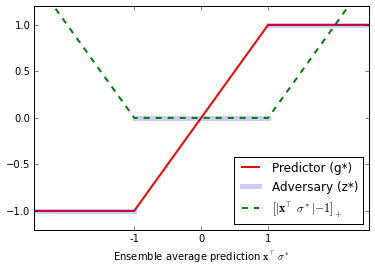
\includegraphics[width=0.55\textwidth]{figs/optstrats.png}
\caption{
\label{fig:optstrats}
The optimal strategies and slack function as a function of the ensemble prediction $\vx^\top \sigma^*$.}
\end{figure}

The proof of this theorem is a standard application of Lagrange duality and the minimax theorem.
The minimax value of the game and the optimal strategy for the predictor $\vg^*$ (Lemma~\ref{lem:game1gopt}) 
are our main objects of study and are completely characterized, 
and the theorem's partial description of $\vz^*$ (proved in Lemma \ref{lem:game1zopt}) 
will suffice for our purposes. 
\footnote{For completeness, Corollary \ref{cor:zoptfullpred} in the appendices 
specifies $z_i^*$ when $\abs{\vx_{i}^\top \sigma^*} = 1$.}

Theorem \ref{thm:gamesolngen} illuminates the importance of the optimal weighting $\sigma^*$ over hypotheses. 
This weighting $\sigma^* \in \argmin_{\sigma \geq 0^p} \gamma (\sigma)$ is the solution 
to a convex optimization problem (Lemma \ref{lem:helperthreshcvx}), 
and therefore we can efficiently compute it and $\vg^*$ to any desired accuracy. 
The ensemble prediction (w.r.t. this weighting) on the test set is $\vF^\top \sigma^*$, 
which is the only dependence of the solution on $\vF$. 

More specifically, the minimax optimal prediction and label \eqref{eqn:opt-strats} on any test set example $\vx_j$ 
can be expressed as functions of the ensemble prediction $\vx_j^\top \sigma^*$ 
on that test point alone, without considering the others. 
The $\vF$-dependent part of the slack function also depends separately on each test point's ensemble prediction. 
Figure \ref{fig:optstrats} depicts these three functions. 

\section{Ball Specialists}

We restrict our attention to a special case which corresponds,
roughly, to nearest neighbor methods.
\begin{enumerate}
  \item The input space is $R^d$.
    The rules that we use are ``specialists'' that are balls. The set
    $\B$ contains all rules of the form 
    \[
    B_{r,\cc,l}(\x) =
    \begin{cases}
      l & \text{if } \| \cc- \x \| \leq r \\
    0 & \text{otherwise }
    \end{cases}
    \]
    Where $r \geq 0$ is the radius of the ball, $\cc \in R^d$ is the
    center of the ball and $l \in \{-1,+1\}$ is the label of the ball.
    We will drop the subscripts of $B$ when clear from context.
  \item
    We use $\vx \in B$ to indicate that $B(\vx) \neq 0$.
  \item
    We denote by $\D$ the distribution of examples $(\vx,y) \sim R^d
    \times \{-1,+1\}$.
  \item
    We denote the {\em probability} of a ball $B$ by $p(B) \doteq
    P_{\D}(\vx \in B)$
  \item
    We use the term {\em bias} of a ball to refer to the conditional
    expectation of the label for a ball by
    $$
    \bias(B) \doteq E_{(\vx,y)\sim\D}\left( l|\vx \in B \right)
    $$
  \item
    Similarly, we define the bias of a particular instance $\vx \in
    R^d$ as
    $$
    \bias(\vx) = E_{(\vx,y)\sim\D}\left( l|\vx \right)
    $$
  \item
    The training sample $T=((x_1,y_1),\ldots,(x_n,y_n))$ is chosen IID
    according to the distribution $\D$. We denote by $\eD$ the
    empirical distribution that is defined by the sample. We denote
    the empirical probability and the empirical bias of the ball $B$
    by $\ep(B)$ and $\ebias(B)$ respectively. Where $\eD$ takes the
    place of $\D$ in the definitions.
  \item
    We define the {\em Bayes optimal} rule for the distribution $\D$
    to be $o(\vx) = \sign(\bias(\vx))$
\end{enumerate}

\section{Conditions}

For any $\Delta,\gamma>0$, we define the set of $(\Delta,\gamma)$-good balls w.r.t. the
distribution $\D$ as
\[
\B_{\Delta,\gamma} = \left\{ B \in \B | p(B) \geq \Delta\;\mbox{ and }
|\bias(B)|\geq \gamma \right\}
\]
\begin{enumerate}
  \item
Consider the instances $\vx_1,\ldots,\vx_n$ paired with their bias:
$S=((\vx_1,\bias(\vx_1)),\ldots,((\vx_n,\bias(\vx_n))$
\item
Consider the matrix $\vF$ that is defined by restricting
$\B_{\Delta,\gamma}$ to $S$. We assume that $\vF$ is invertible. In
other words, that for any $\vz$ there exists $\vb$ such that $\vF \vz'
= \vb$ if and only if $\vz=\vz'$
\item
We say that a point $\vx$ {\em conforms} with a ball $B \in
\B_{\Delta,\gamma}$ if $\vx \in  B$ and $\bias(B) \bias(\vx)>0$
\item
We say that a point $\vx$ is {\em good} if for all balls $B$ such that $\vx
\in B \in \B_{\Delta,\gamma}$, either $\vx$ conforms with $B$ or there
is another ball $\vx \in C \in \B_{\Delta,\gamma}$ such that $C
\subset B$ and $\vx$ conforms with $C$
\end{enumerate}



\end{document}
